\section{Sécurité}

\subsection{Contrôle d'accès}
Cette application web est destinée à être utilisée par plusieurs personnes avec des rôles différents au sein de la société. Chaque rôle n'a pas les mêmes droit quant à la consultation ou manipulation des données de l'application. On peut ainsi distinguer cinq catégories d'utilisateurs: 
\begin{enumerate}
  \item \textbf{Inconnu}: utilisateur non-authentifié. Celui-ci n'a aucun droit sur les données et peut uniquement accèder à la page de connexion de l'application. 
  \item \textbf{Comptabilité}: 
  \begin{itemize}
    \item peut se connecter
    \item peut uniquement consulter l'ensemble des données 
    \item peut générer des pdf (factures, commandes, ...)
  \end{itemize}
  \item \textbf{Atelier}: 
  \begin{itemize}
    \item a tous les droits de la comptabilité
    \item peut créer/modifier une fiche de travail
    \item peut créer/modifier une commande
  \end{itemize}
  \item \textbf{Administration}: 
  \begin{itemize}
    \item peut tout faire hormis supprimer les utilisateurs de type "Développeur"
  \end{itemize}
  \item \textbf{Développeur}: 
  \begin{itemize}
    \item peut tout faire et a accès aux logs et métriques
  \end{itemize}
\end{enumerate}

\newpara

Afin d'authentifier un utilisateur et donc de lui donner certains droits ou non, l'application utilise des JSON Web Tokens (JWT)\footnote{Comment cela fonctionne-t-il? Explication en vidéo: \url{https://www.youtube.com/watch?v=7Q17ubqLfaM}}. Les tokens sont générés lors de chaque nouvelle connexion réussie et sont valides pendant 48h. Toute action effectuée à l'aide d'un token non-valide déconnecte automatiquement l'utilisateur et le re-dirige vers la page de connexion. 

\newpage

\subsection{Hachage et Chiffrement}

Avant toute chose il me semble bon de rappeler la différence entre le \textbf{hachage} et le \textbf{chiffrement}: 
\begin{itemize}
  \item \textbf{hachager}: \\ Utilisation d'un algorithme de hachage uni-directionnel afin de transformer les données de manière irréversible et de longueur fixe. Il est donc possible de comparer deux "hash".
  \item \textbf{chiffrer}: \\ Encoder des données afin qu'uniquement la personne ayant la clé de déchiffrement puisse les déchiffrer. Cette action est donc réversible.
\end{itemize}

\subsubsection{Données enregistrées}
Toute donnée susceptible d'être un risque pour l'intégrité et la protection de l'application ou des autres données est stockée sous forme de "hash" (et non en clair\footnote{lisible et comprehensible par quiconque}) dans la base de données (par exemple les mots de passes des utilisateurs). 

\newpara

Afin de hacher ces données, j'ai utilisé la librairie "bcrypt". La librairie "bcrypt" est une des librairies de hachage les plus réputées. Elle permet d'incorporer un sel (salt)\footnote{\textit{"Le salage, est une méthode permettant de renforcer la sécurité des informations qui sont destinées à être hachées (par exemple des mots de passe) en y ajoutant une donnée supplémentaire afin d’empêcher que deux informations identiques conduisent à la même empreinte (la résultante d’une fonction de hachage)"}\cite{Salt}} afin de se protéger contre les attaques par table de correspondance (rainbow table)\footnote{Attaque consistant à comparer un "hash" à un table reprenant un grand nombre de paires de text clair et le "hash" correspondant.}. De plus elle est facilement paramétrable permettant ainsi d'augmenter la complexité de l'algorithme utilisé afin de palier aux attaques par force brute\footnote{Attaque consistant à essayer un grand nombre de donnés générées automatiquement en espérant trouver la bonne.} utilisant des machines à puissances de calcule importante. 

\subsubsection{HTTPS}
Stocker les données à risque de manière chiffrée dans la base de données est une chose, cependant, avant que les données n'arrivent jusque là elles sont potentiellement envoyées en clair sur le réseau (internet). Afin d'éviter cela, je n'autorise que les connexion HTTPS et redirige les connexions HTTP vers le HTTPS. Ceci permet de garantir que l'entièreté des données envoyées sont chiffrées et dès lors beaucoup moins vulnérables aux attaques de type "Man In The Middle" (MITM).

\newpage

\subsection{HTTP Headers}

Les headers HTTP permettent de sécuriser un site-web contre la plupart des attaques les plus répandues et ce de manière relativement simple. Voici en résumé les principaux headers que j'ai configurés:

\begin{itemize}
  \item \textbf{Strict-Transport-Policy (STP)}: \\ Header permettant d'indiquer au navigateur que le site-web ne peut être accèdé qu'en utilisant HTTPS au lieu de HTTP. \\
  
  \item \textbf{Content-Security-Policy (CSP)}: \\ \textit{"L'en-tête de réponse HTTP Content-Security-Policy permet aux administrateurs d'un site web de contrôler les ressources que l'agent utilisateur est autorisé à charger pour une page donnée. Bien qu'il y ait quelques exceptions, ces règles impliquent la plupart du temps de définir les origines du serveur et les points d'accès pour les scripts. Cet en-tête aide à se protéger contre les attaques de cross-site scripting."}\cite{CSP} \\

  \item \textbf{X-Frame-Options}: \\ \textit{"L'en-tête de réponse HTTP X-Frame-Options peut être utilisé afin d'indiquer si un navigateur devrait être autorisé à afficher une page au sein d'un élément <frame>, <iframe>, <embed> ou <object>. Les sites peuvent utiliser cet en-tête afin d'éviter les attaques de clickjacking pour s'assurer que leur contenu ne soit pas embarqués dans d'autres sites."}\cite{X-Frame} \\

  \item \textbf{X-Content-Type-Policy}: \\ \textit{"L'entête X-Content-Type-Options est un marqueur utilisé par le serveur pour indiquer que les types MIME annoncés dans les en-têtes Content-Type ne doivent pas être modifiés ou et suivis. Cela permet de se détacher du sniffing de type MIME, ou, en d'autres termes, c'est une façon de dire que les webmasters savaient ce qu'ils faisaient."}\cite{X-Content}
\end{itemize}

\newpara

Après avoir configuré ces différents headers, j'ai testé le bon fonctionnement de ceux-ci en lançant une analyse en ligne. Comme le montre la \textit{figure \ref{Headers}} l'ensemble des headers ont bien été configurés et protègent désormais le site-web. 

\begin{figure}[H]
  \centering
  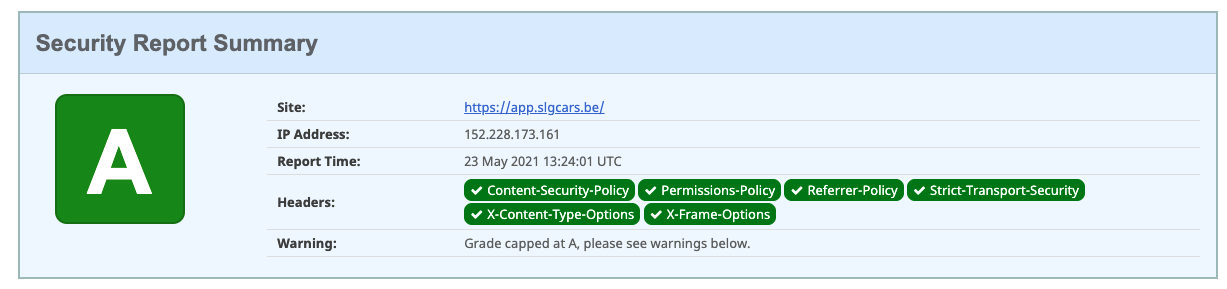
\includegraphics[width=\linewidth]{img/securityHeaders.png}
  \caption{Résultat analyse de sécurité des headers fait sur \url{https://securityheaders.com/}}
  \label{Headers}
\end{figure}

\newpage 

\subsection{Dependabot Github}

Durant le développement de l'application, afin de ne pas réinventer la roue, il est fréquent d'utiliser des packages/composants externes créés par d'autres développeurs. Ces packages étant utilisés par un grand nombre d'utilisateurs, ils sont une proie "facile" pour des personnes malveillantes qui souhaiteraient infecter un grand nombre de site-web. Ces packages sont dès lors régulièrement mis à jour par les créateurs afin de garantir une sécurité maximale. 

\newpara 

Mais comment savoir quand une nouvelle version d'un package est disponible pour des raisons de sécurité? Heureusement, Github propose plusieurs services permettant de réaliser des analyses de sécurité statique sur le code y étant hébergé. Ainsi j'ai utilisé "Dependabot" qui scanne périodiquement l'ensemble des dépendances du projet afin d'y déceler de potentielles failles. Si celui-ci en trouve, il m'envoie un email me prévenant de la nature de la faille et de sa dangerosité. Il ne me reste alors plus qu'a mettre à jour manuellement le(s) package(s) concerné(s) ou d'accepter une pull-request\footnote{Demande de modification du code source par une tierce personne. Pour plus d'information, voir: \url{https://www.atlassian.com/git/tutorials/making-a-pull-request}} générée par "Dependabot".

\newpara

\begin{figure}[H]
  \centering
  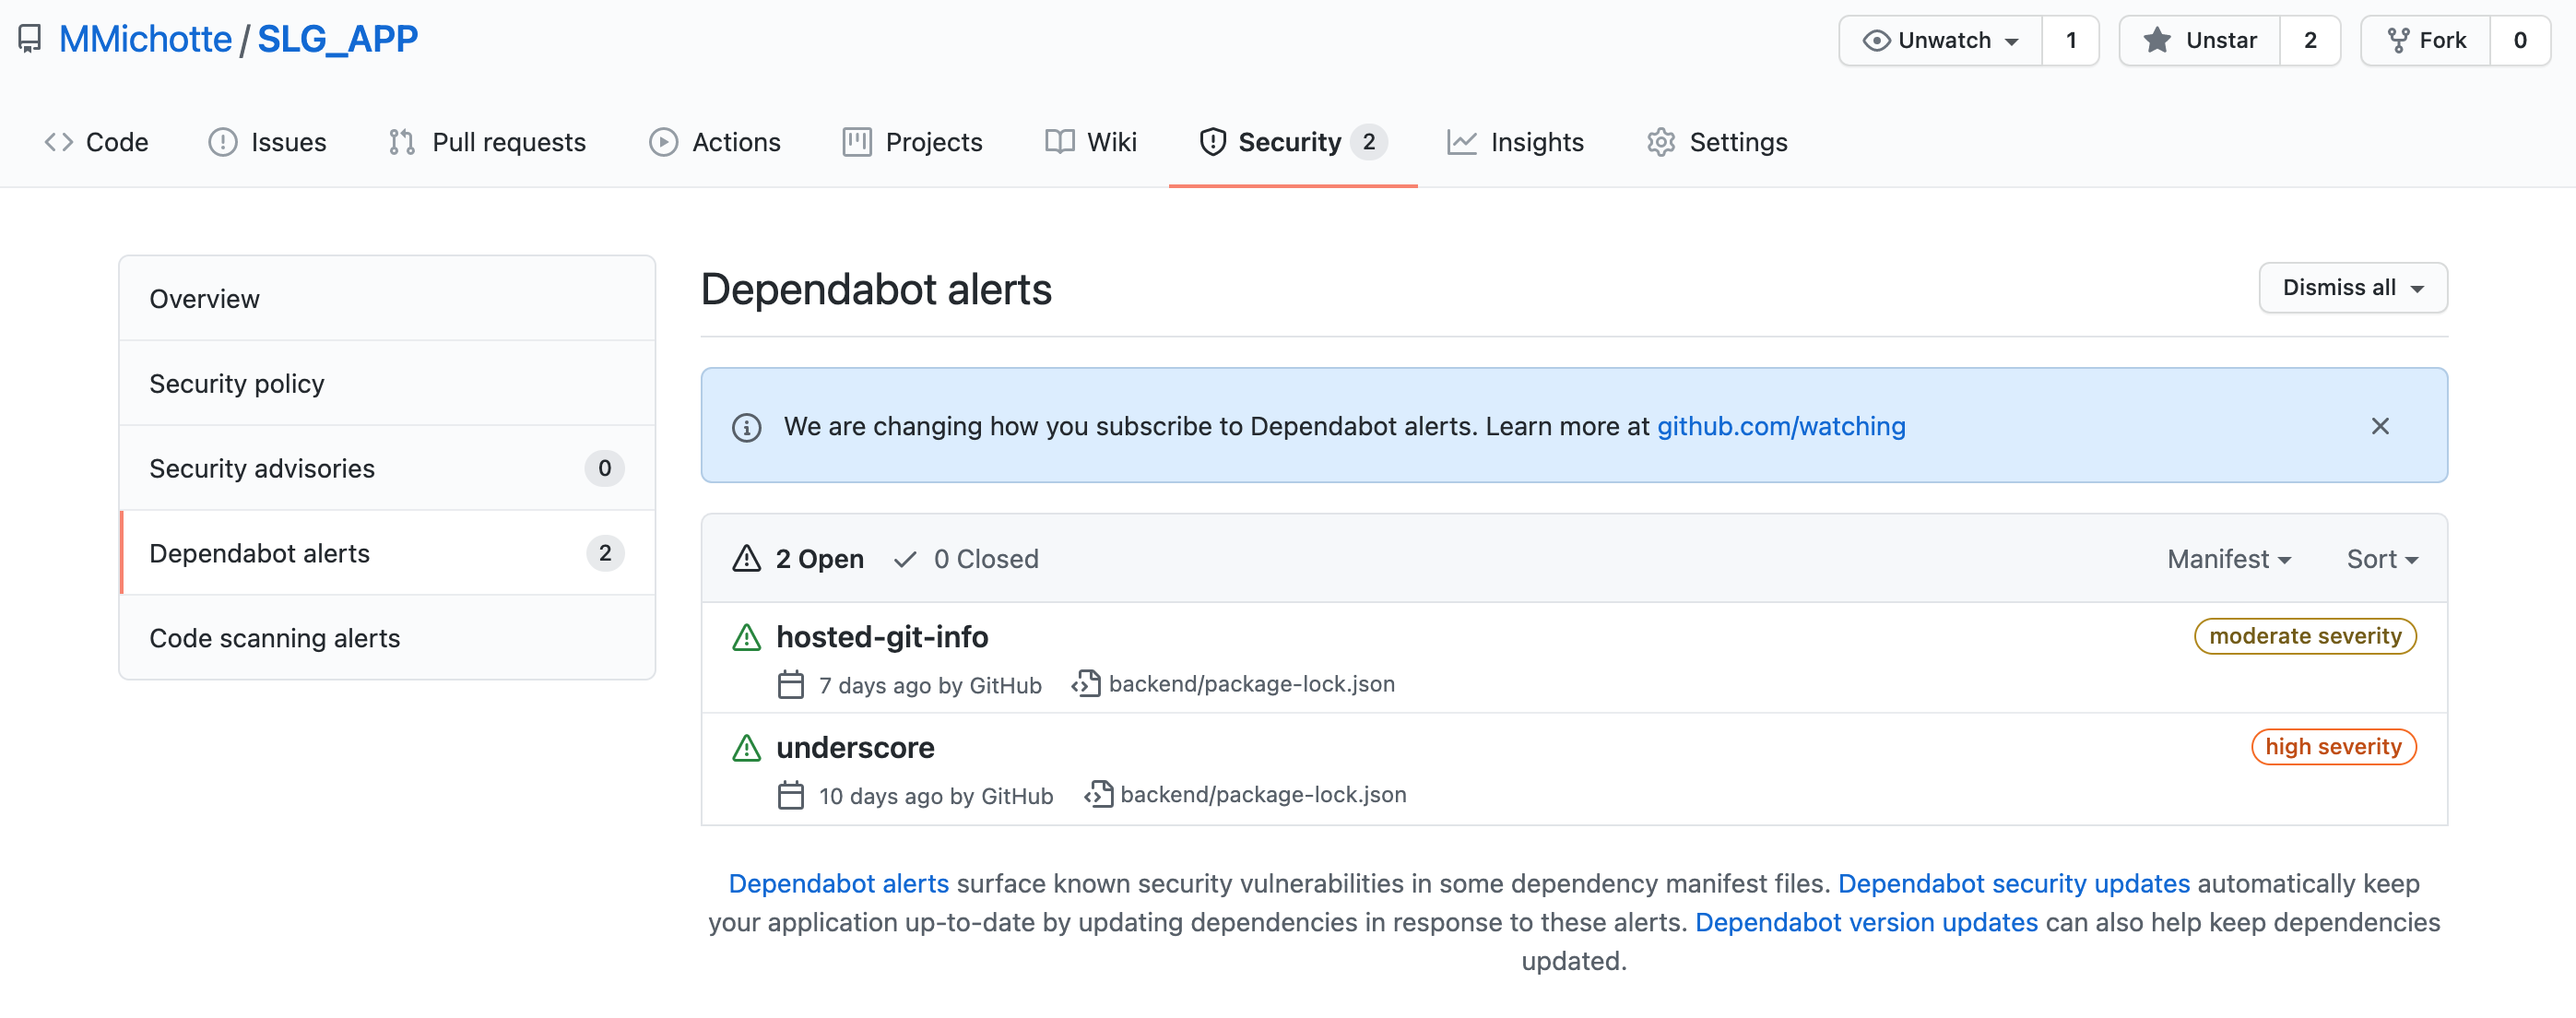
\includegraphics[width=\linewidth]{img/dependabot.png}
  \caption{Exemple d'alertes générées par "Dependabot"}
\end{figure}